
% \section{Solenoidal magnet}


% %%%%%% SLIDE
% \begin{frame}{\textcolor{Goldenrod}{Solenoidal Magnet }}
%   \(
%   \<{0.45\textwidth}
%   \img{26_magnet_solonoid.pdf}
%   \>
%   \<{0.7\textwidth}
%   \itt
% \item[$\Box$]<1-> to optimize the momentum resolution, $\delta p_T /p_T$ and tracking
%   pattern recognition $\to $ a central field of $2 T$
% \item[$\Box$]<2-> design criteria:
%   \itt
% \item [$i)$] to operate safely and stably at either polarity
% \item [$ii)$] a uniform field over as large a percentage of the volume as practical,
% \item [$iii)$] as thin as possible to make the tracking volume as large as possible,
% \item [$iv)$] an overall thickness of approximately $1 X_0$ at $\eta = 0$ to optimize
%   the performance of the central preshower detector mounted on the outside of
%   the solenoid cryostat.
%   \tti
%   \tti
%   \>
%   \)
% \end{frame}

% \subsection{Magnetic construction}
% %%%%%% SLIDE
% \begin{frame}{\textcolor{Goldenrod}{Solenoidal Magnet }}
%     \begin{figure}[h]
%       \centering
%       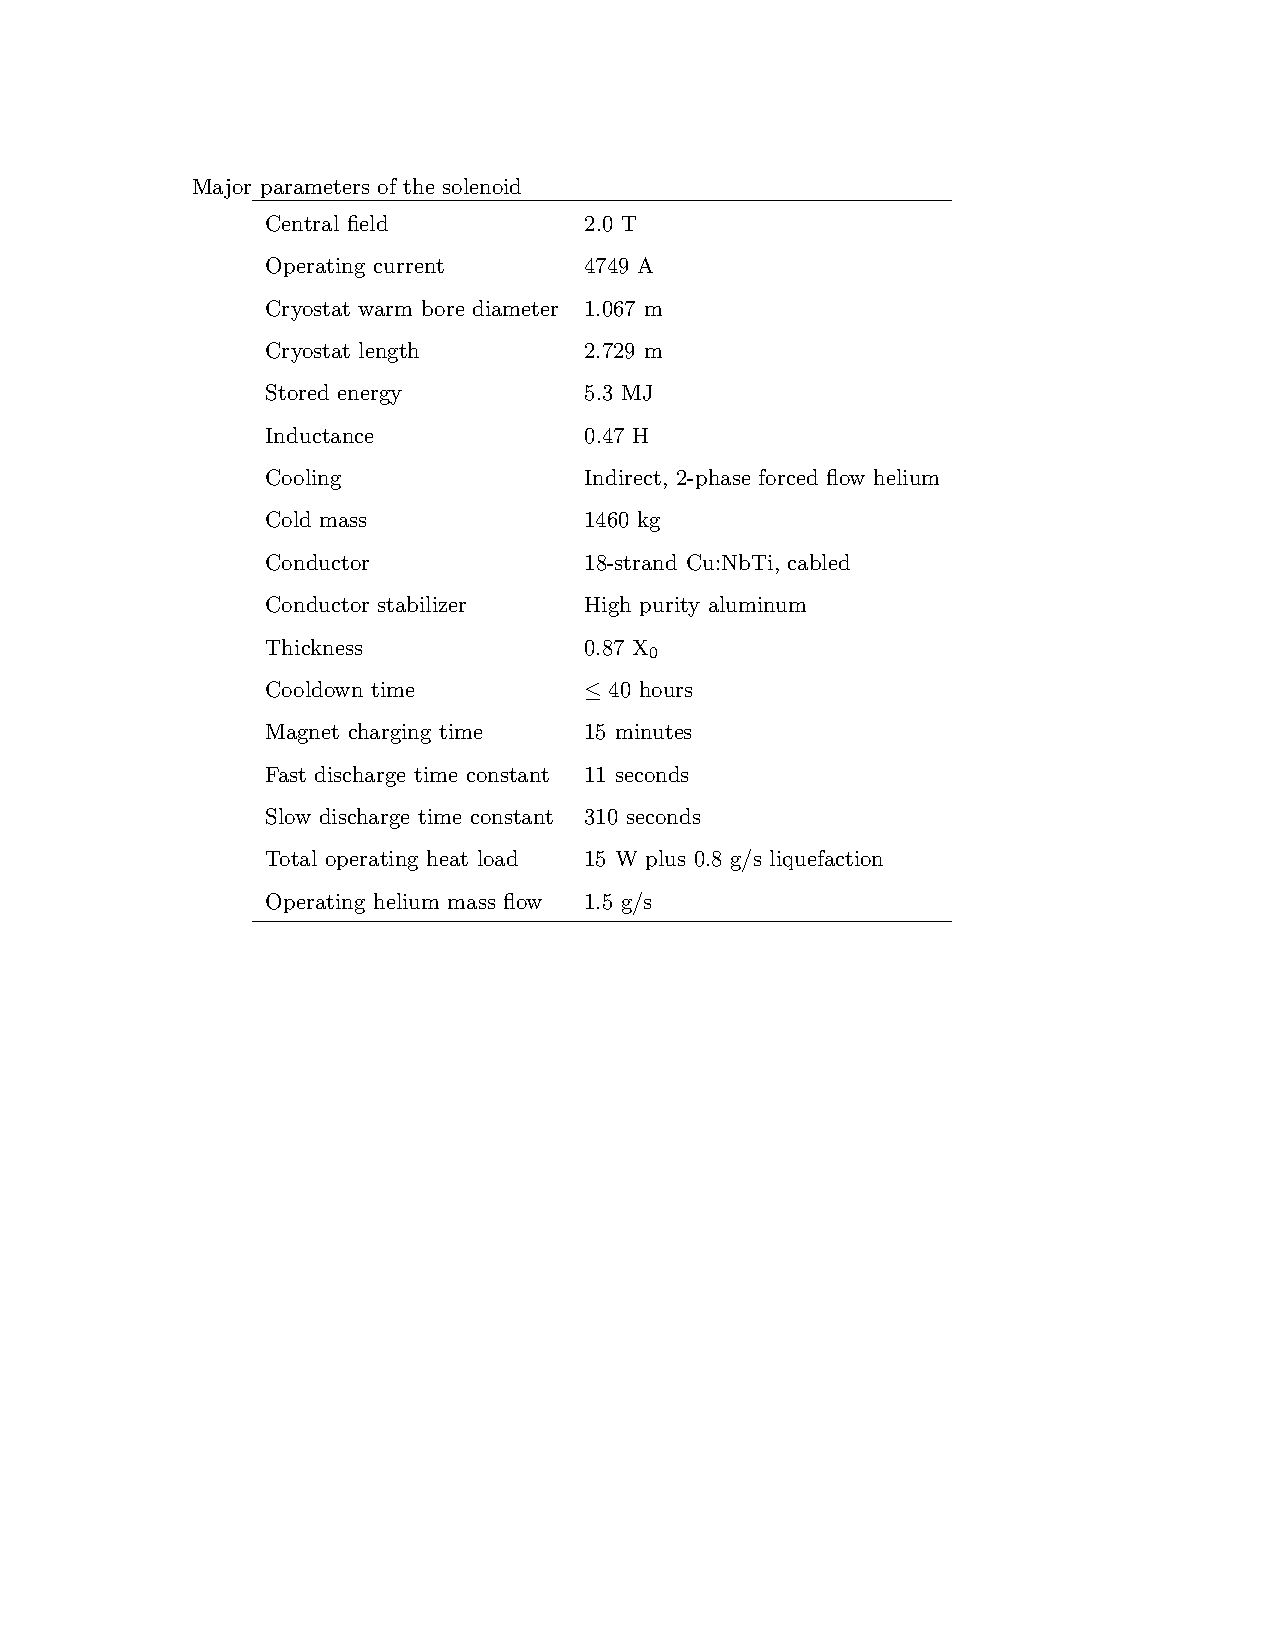
\includegraphics[height=0.6\textheight]{./Images/25_magnet_solonoid.pdf}
%       \caption*{The solenoid is wound with two layers of superconductor to achieve the required
%         linear current density for a $2 T$ central field.}
%     \end{figure}
    
% \end{frame}

% \subsection{Magnetic field}
% %%%%%% SLIDE
% \begin{frame}{\textcolor{Goldenrod}{Magnet Field}}
%   \(
%   \<{0.55\textwidth}
%   \itt[<+->]
% \item Within the solenoid (operated
%   at $4749 A$), The calculated magnetic field is scaled by 0.09\%
%   to agree with the measurement.
% \item Within the toroid (operated at $1500 A$)
%   The calculated magnetic field is scaled by $4.3\%$
%   \tti
%   \>
%   \<{0.6\textwidth}
%   \img{28_magnet_solonoid.pdf}\\
%   {\scriptsize The $y-z$ view of the $D\emptyset$ magnetic field (in
%     $kG$). The field
%     in the central toroid is approximately $1.8 T$}
%   \note{with both the toroidal
%     and solenoidal magnets at full current ($1500 A$ and $4749 A$, respectively).}
%   \>
%   \)
% \end{frame}
